\documentclass[11pt,letter]{article}\usepackage[]{graphicx}\usepackage[]{color}
%% maxwidth is the original width if it is less than linewidth
%% otherwise use linewidth (to make sure the graphics do not exceed the margin)
\makeatletter
\def\maxwidth{ %
  \ifdim\Gin@nat@width>\linewidth
    \linewidth
  \else
    \Gin@nat@width
  \fi
}
\makeatother

\definecolor{fgcolor}{rgb}{0.345, 0.345, 0.345}
\newcommand{\hlnum}[1]{\textcolor[rgb]{0.686,0.059,0.569}{#1}}%
\newcommand{\hlstr}[1]{\textcolor[rgb]{0.192,0.494,0.8}{#1}}%
\newcommand{\hlcom}[1]{\textcolor[rgb]{0.678,0.584,0.686}{\textit{#1}}}%
\newcommand{\hlopt}[1]{\textcolor[rgb]{0,0,0}{#1}}%
\newcommand{\hlstd}[1]{\textcolor[rgb]{0.345,0.345,0.345}{#1}}%
\newcommand{\hlkwa}[1]{\textcolor[rgb]{0.161,0.373,0.58}{\textbf{#1}}}%
\newcommand{\hlkwb}[1]{\textcolor[rgb]{0.69,0.353,0.396}{#1}}%
\newcommand{\hlkwc}[1]{\textcolor[rgb]{0.333,0.667,0.333}{#1}}%
\newcommand{\hlkwd}[1]{\textcolor[rgb]{0.737,0.353,0.396}{\textbf{#1}}}%
\let\hlipl\hlkwb

\usepackage{framed}
\makeatletter
\newenvironment{kframe}{%
 \def\at@end@of@kframe{}%
 \ifinner\ifhmode%
  \def\at@end@of@kframe{\end{minipage}}%
  \begin{minipage}{\columnwidth}%
 \fi\fi%
 \def\FrameCommand##1{\hskip\@totalleftmargin \hskip-\fboxsep
 \colorbox{shadecolor}{##1}\hskip-\fboxsep
     % There is no \\@totalrightmargin, so:
     \hskip-\linewidth \hskip-\@totalleftmargin \hskip\columnwidth}%
 \MakeFramed {\advance\hsize-\width
   \@totalleftmargin\z@ \linewidth\hsize
   \@setminipage}}%
 {\par\unskip\endMakeFramed%
 \at@end@of@kframe}
\makeatother

\definecolor{shadecolor}{rgb}{.97, .97, .97}
\definecolor{messagecolor}{rgb}{0, 0, 0}
\definecolor{warningcolor}{rgb}{1, 0, 1}
\definecolor{errorcolor}{rgb}{1, 0, 0}
\newenvironment{knitrout}{}{} % an empty environment to be redefined in TeX

\usepackage{alltt}    
%\usepackage[latin1]{inputenc}
\usepackage[parfill]{parskip} % Activate to begin paragraphs with an empty line rather than an indent
\usepackage{amsmath,amsthm,amssymb,bbm} %math stuff
\usepackage{ctable}
\usepackage{placeins} % FloatBarrier
\usepackage{fancyhdr}
\usepackage{lastpage}
\usepackage{float}    % for fig.pos='H'
\usepackage{rotfloat} % for sidewaysfigure
%\usepackage{subfig}   % for subfigure
\usepackage{subcaption}  % an alternative package for sub figures
\newcommand{\subfloat}[2][need a sub-caption]{\subcaptionbox{#1}{#2}}
\usepackage{comment}
\usepackage[round]{natbib}   % omit 'round' option if you prefer square brackets
\bibliographystyle{plainnat}
\usepackage{setspace} %Spacing
\usepackage{graphicx,graphics}
\usepackage{booktabs,tabularx}
\usepackage{enumerate}
\usepackage{makecell}
\usepackage{xfrac}
\usepackage{color, colortbl, xcolor}
\usepackage{booktabs,dcolumn} % for use with texreg in R
\usepackage[pagebackref=true,bookmarks]{hyperref}
\hypersetup{
    unicode=false,          
    pdftoolbar=true,        
    pdfmenubar=true,        
    pdffitwindow=false,     % window fit to page when opened
    pdfstartview={FitH},    % fits the width of the page to the window
    pdftitle={004-Figures},    % title
    pdfauthor={SRB},     % author
    pdfsubject={Subject},   % subject of the document
    pdfcreator={SRB},   % creator of the document
    pdfproducer={SRB}, % producer of the document
    pdfkeywords={}, % list of keywords
    pdfnewwindow=true,      % links in new window
    colorlinks=true,       % false: boxed links; true: colored links
    linkcolor=red,          % color of internal links (change box color with linkbordercolor)
    citecolor=blue,        % color of links to bibliography
    filecolor=black,      % color of file links
    urlcolor=cyan           % color of external links
}

% my commands
\newcommand{\tm}[1]{\textrm{#1}}


% fancy header commands
\renewcommand{\headrulewidth}{0.0pt}
\renewcommand{\footrulewidth}{0.0pt}
\setlength{\textheight}{9.00in}
\setlength{\textwidth}{7.00in}
\setlength{\topmargin}{-0.5in}
\setlength{\evensidemargin}{-0.25in}
\setlength{\oddsidemargin}{-0.25in}
\renewcommand{\baselinestretch}{1.2}
\makeatletter
\makeatother
\lfoot{} \cfoot{ } \rfoot{{\small{\em Page \thepage \ of \pageref{LastPage}}}}
\IfFileExists{upquote.sty}{\usepackage{upquote}}{}
\begin{document}
\pagestyle{fancy}

\title{004-Figures}
\author{Attitudes Towards Abortion\thanks{Thanks to Gillian Ainsworth, Zhuoyu Wang and Yishu Wang for providing this example}}
\maketitle








\begin{abstract}
Exploratory data analysis is a crucial first step in answering a scientific question. In this document I provide some examples of how to dynamically include figures in reports. Several figure chunk options that \texttt{knitr}~\citep{k1,k2,k3} provides are discussed. We illustrate these options along with the plotting capabilities of \texttt{ggplot2}~\citep{ggplot2} and \texttt{lattice}~\citep{lattice}. The data come from part of an investigation of British Social Attitudes (BSA) Survey~\citep{mcgrath1986british} started in 1983. Every participant was asked whether they supported or opposed a woman's right to have an abortion under seven different circumstances each year from 1983 to 1986. We are interested in assessing the impact of gender, age, self assessed social class, political party, and religion on one's attitude towards abortion, and find out what are the main factors that affect people's attitude towards abortion.  We are also interested in assessing whether people's attitude towards abortion have changed over the years, and whether these changes are due to time or the change of some other factors.  
\end{abstract}


\section{Background}

The respondents were asked if they supported or opposed a woman's right to have an abortion under seven different circumstances.   The same seven circumstances were presented in each of the four years of the study, and show different situations. A higher score indicates a more positive attitude towards abortion. The seven circumstances are as follows:

\begin{itemize}
\item[1] The woman decides on her own she does not wish to have the child.  
\item[2] The couple agree they do not wish to have the child.  
\item[3] The woman is not married and does not wish to marry the man.  
\item[4] The couple cannot afford any more children.  
\item[5] There is a strong chance of a defect in the baby.  
\item[6] The woman's health is seriously endangered by the pregnancy.  
\item[7] The woman became pregnant as a result of rape.  
\end{itemize}



\section{Exploratory Analysis}






Figure~\ref{fig:figure-1} shows the response by each variable, ignoring the repeated measurement structure in the data set.  The plot of response by age suggests that the association between the response and age is not linear.  Basically, younger group tends to have higher scores than older group.  We also see a big drop in positive attitudes towards abortion in 1984 and then an increase in subsequent years.  There also seems to be quite a bit of variability in the scores as a function of religion.  No difference was observed between males and females, between political party or social class.

\begin{knitrout}
\definecolor{shadecolor}{rgb}{0.969, 0.969, 0.969}\color{fgcolor}\begin{figure}[H]

{\centering 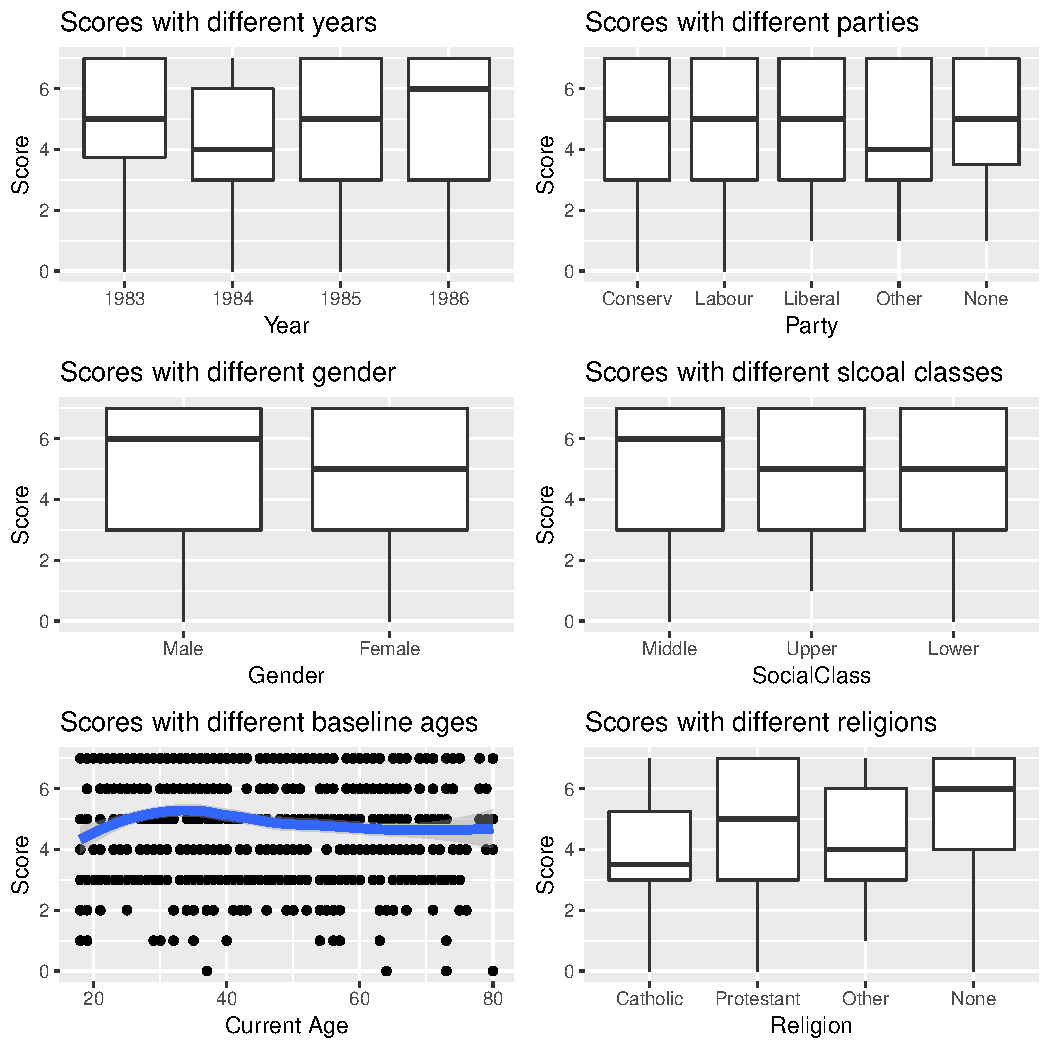
\includegraphics[width=\maxwidth]{figure/figure-1-1} 

}

\caption[The response by each variable, ignoring the repeated measurement structure in the data set]{The response by each variable, ignoring the repeated measurement structure in the data set}\label{fig:figure-1}
\end{figure}


\end{knitrout}




Figure~\ref{fig:figure-2} shows the observed response profiles of a random sample of 30 subjects (Figure~\ref{fig:figure-21}) with the corresponding OLS fits (Figure~\ref{fig:figure-22}) as a function of year.  Much variation can be observed in the initial scores, but on average, the scores decrease from 1983 to 1984, and then increase in the last two years.   We should keep in mind that there are some ties in the plot.

\begin{knitrout}
\definecolor{shadecolor}{rgb}{0.969, 0.969, 0.969}\color{fgcolor}\begin{kframe}
\begin{alltt}
\hlkwd{set.seed}\hlstd{(}\hlnum{123455}\hlstd{)}
\hlstd{sample.id} \hlkwb{<-} \hlkwd{sample}\hlstd{(}\hlkwd{unique}\hlstd{(DT}\hlopt{$}\hlstd{id),} \hlnum{30}\hlstd{)}
\hlkwd{xyplot}\hlstd{(answers} \hlopt{~} \hlkwd{factor}\hlstd{(year),} \hlkwc{group} \hlstd{= id,} \hlkwc{data} \hlstd{= DT[id} \hlopt
    \hlstd{sample.id],} \hlkwc{type} \hlstd{=} \hlkwd{c}\hlstd{(}\hlstr{"l"}\hlstd{,} \hlstr{"p"}\hlstd{),} \hlkwc{lty} \hlstd{=} \hlnum{2}\hlstd{,} \hlkwc{xlab} \hlstd{=} \hlstr{"year"}\hlstd{,} \hlkwc{ylab} \hlstd{=} \hlstr{"score"}\hlstd{,}
    \hlkwc{aspect} \hlstd{=} \hlstr{"xy"}\hlstd{,} \hlkwc{main} \hlstd{=} \hlstr{"response profiles for a random sample of 30 subjects"}\hlstd{)}
\hlkwd{xyplot}\hlstd{(answers} \hlopt{~} \hlkwd{factor}\hlstd{(year),} \hlkwc{group} \hlstd{= id,} \hlkwc{data} \hlstd{= DT[id} \hlopt
    \hlstd{sample.id],} \hlkwc{type} \hlstd{=} \hlkwd{c}\hlstd{(}\hlstr{"r"}\hlstd{),} \hlkwc{aspect} \hlstd{=} \hlstr{"xy"}\hlstd{,} \hlkwc{xlab} \hlstd{=} \hlstr{"year"}\hlstd{,}
    \hlkwc{ylab} \hlstd{=} \hlstr{"score"}\hlstd{,} \hlkwc{index.cond} \hlstd{=} \hlkwa{function}\hlstd{(}\hlkwc{x}\hlstd{,} \hlkwc{y}\hlstd{)} \hlkwd{coef}\hlstd{(}\hlkwd{lm}\hlstd{(y} \hlopt{~} \hlstd{x))[}\hlnum{1}\hlstd{],}
    \hlkwc{main} \hlstd{=} \hlstr{"Least squares fits (with year) for the same random sample of 30 subjects"}\hlstd{)}
\end{alltt}
\end{kframe}\begin{figure}[H]
\subfloat[scores for a random sample of 30 subjects\label{fig:figure-21}]{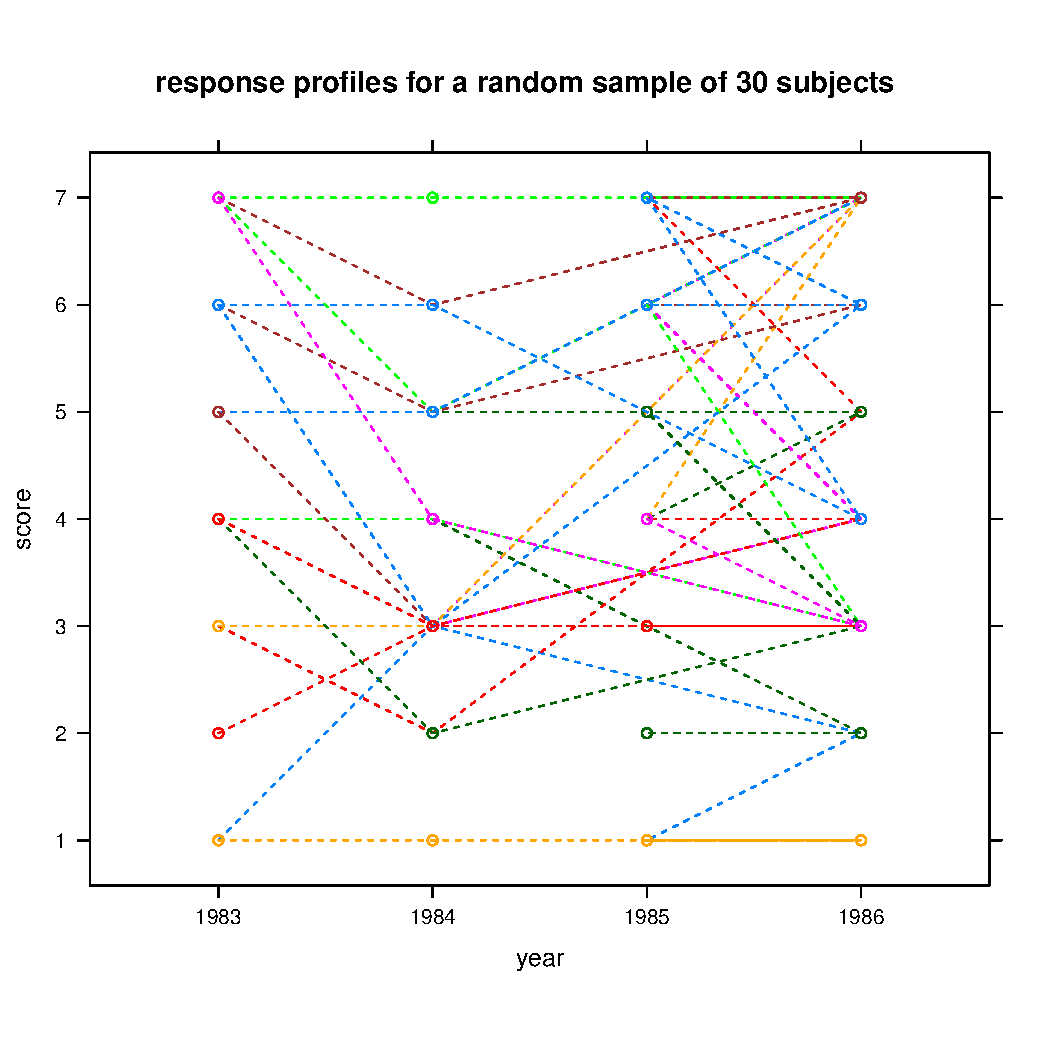
\includegraphics[width=.49\linewidth]{figure/figure-2-1} }
\subfloat[Least squares fits (with year) for same random sample of 30\label{fig:figure-22}]{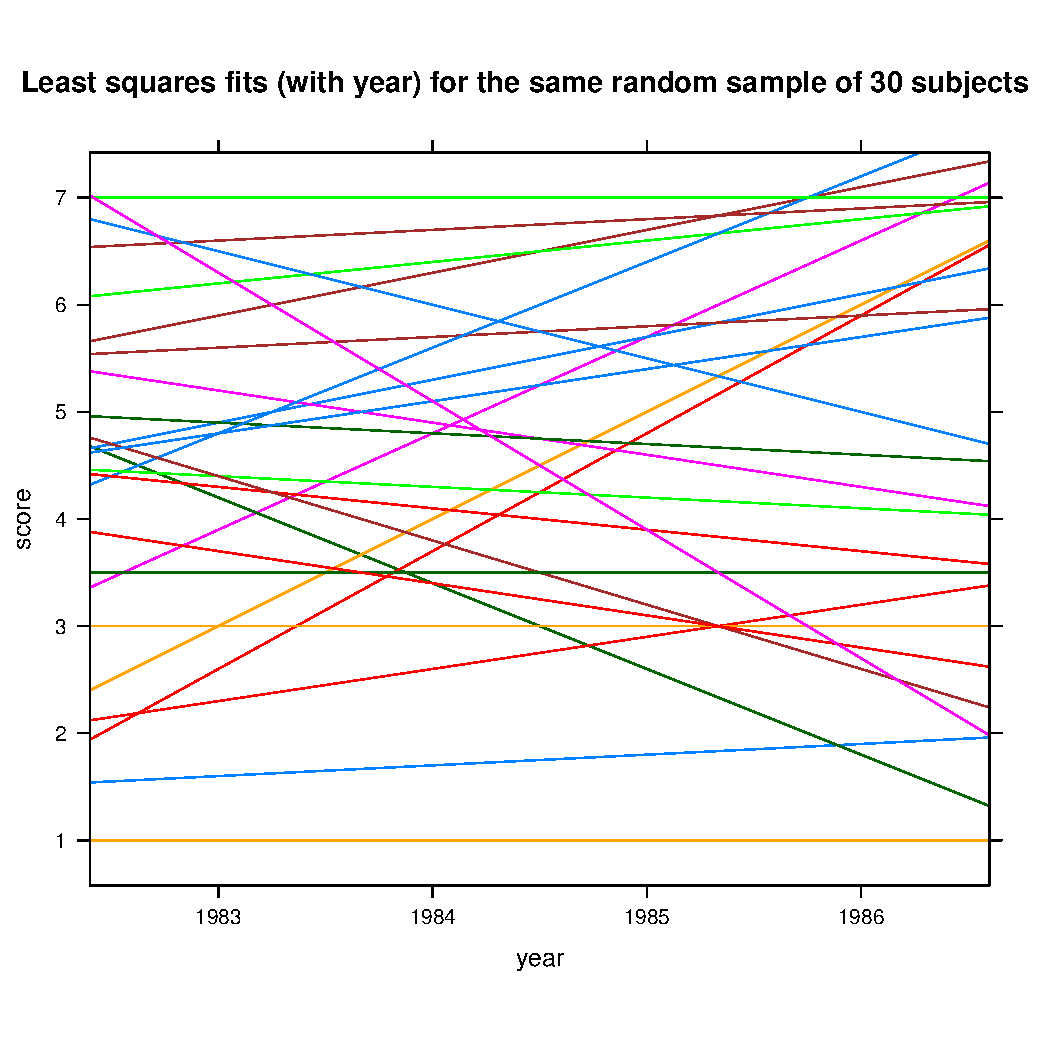
\includegraphics[width=.49\linewidth]{figure/figure-2-2} }\caption[Selected individual score profiles from the British Social Attitudes (BSA) Survey]{Selected individual score profiles from the British Social Attitudes (BSA) Survey}\label{fig:figure-2}
\end{figure}


\end{knitrout}

In Figures~\ref{fig:figure-31}, \ref{fig:figure-32} and~\ref{fig:figure-33} we present the densities of the response by year and political party, self assessed social class and religion, respectively.  Figure~\ref{fig:figure-31} does not show any noticeable change across time and political party though there is an empty cell in 1986.  In Figure~\ref{fig:figure-32}, we observe lower scores in 1984, but the pattern across years and social classes looks similar.  Considering Figure ~\ref{fig:figure-33}, those subject who did not identify with a particular religion tended to answer more positively toward abortion when compared to those subject who were religious. This difference was consistent across all years of the study. 

\begin{knitrout}
\definecolor{shadecolor}{rgb}{0.969, 0.969, 0.969}\color{fgcolor}\begin{figure}[H]

{\centering 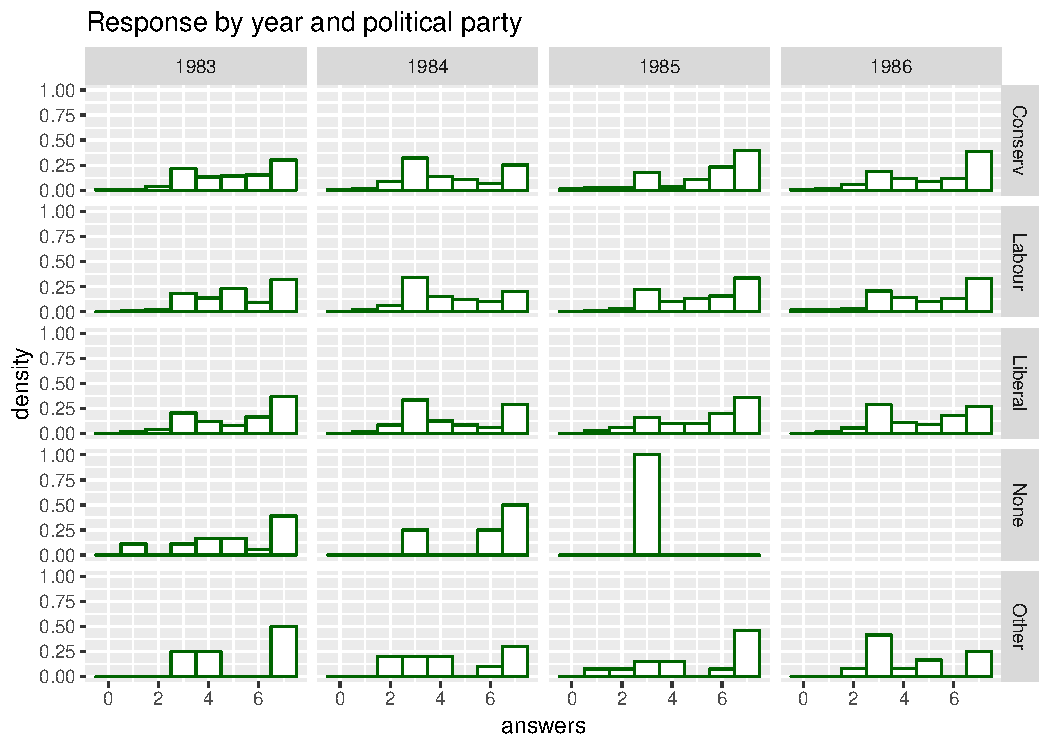
\includegraphics[width=\maxwidth]{figure/figure-3-1} 

}

\caption[Histogram of responses, stratified by year and political party]{Histogram of responses, stratified by year and political party}\label{fig:figure-31}
\end{figure}

\begin{figure}[H]

{\centering 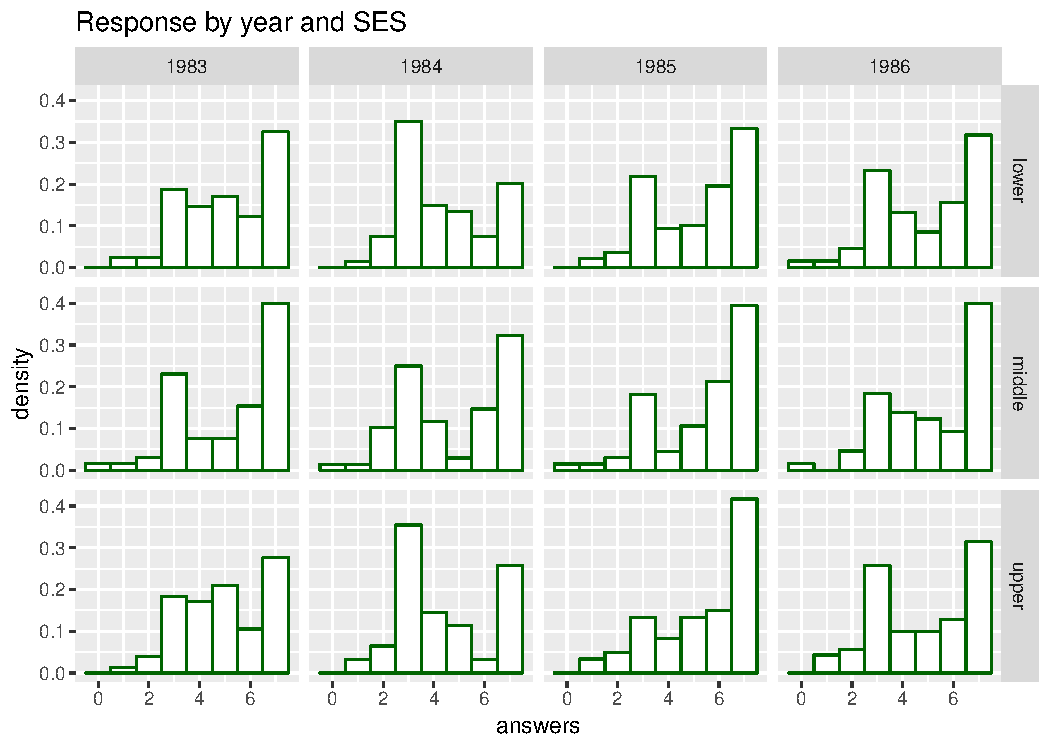
\includegraphics[width=\maxwidth]{figure/figure-3-2} 

}

\caption[The response by year and SES]{The response by year and SES}\label{fig:figure-32}
\end{figure}

\begin{figure}[H]

{\centering 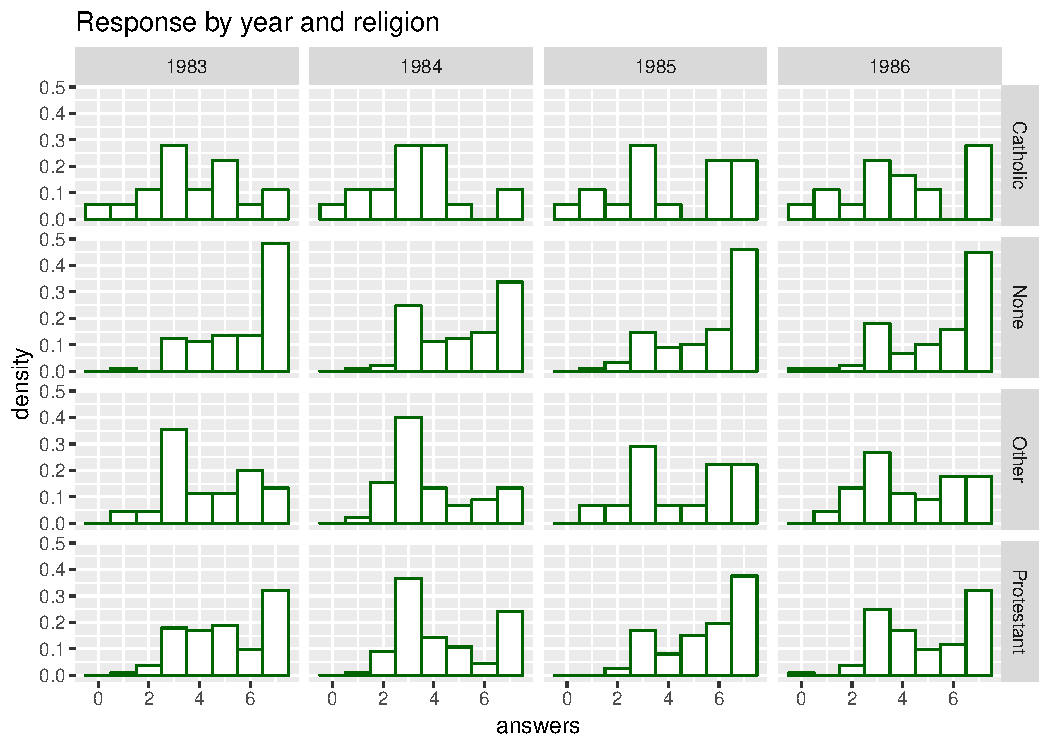
\includegraphics[width=\maxwidth]{figure/figure-3-3} 

}

\caption[The response by year and religion]{The response by year and religion}\label{fig:figure-33}
\end{figure}


\end{knitrout}


We plot answers as a function of age (Figure~\ref{f:figure-61}) with a loess smoothed line (Figure~\ref{f:figure-62}) 

\begin{knitrout}
\definecolor{shadecolor}{rgb}{0.969, 0.969, 0.969}\color{fgcolor}\begin{kframe}
\begin{alltt}
\hlkwd{plot}\hlstd{(DT}\hlopt{$}\hlstd{age, DT}\hlopt{$}\hlstd{answers)}
\end{alltt}
\end{kframe}\begin{figure}[H]

{\centering 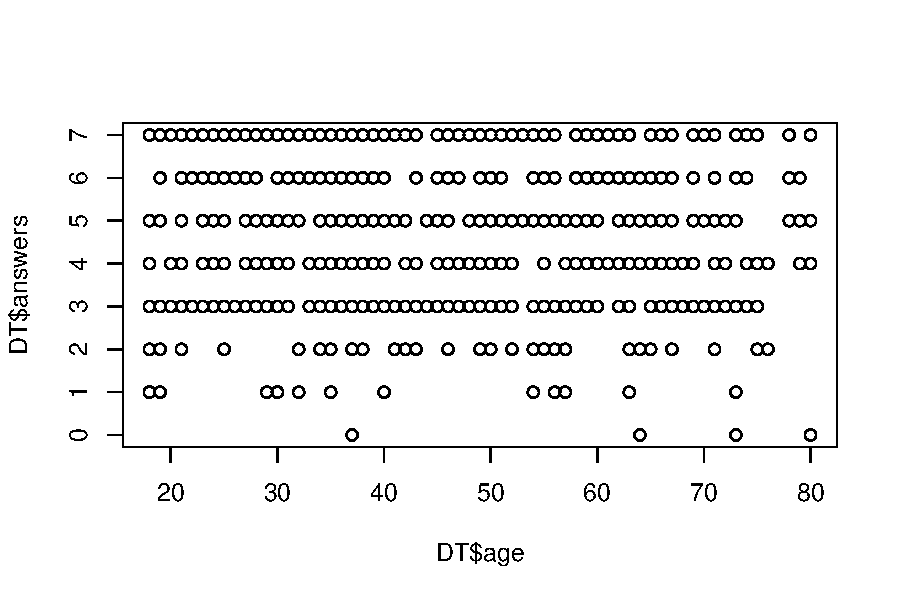
\includegraphics[width=\maxwidth]{figure/figure-6-1} 

}

\caption[Answers vs]{Answers vs. Age}\label{f:figure-61}
\end{figure}

\begin{kframe}\begin{alltt}
\hlkwd{lines}\hlstd{(stats}\hlopt{::}\hlkwd{lowess}\hlstd{(DT}\hlopt{$}\hlstd{age, DT}\hlopt{$}\hlstd{answers),} \hlkwc{col} \hlstd{=} \hlstr{"red"}\hlstd{,} \hlkwc{lwd} \hlstd{=} \hlnum{3}\hlstd{)}
\end{alltt}
\end{kframe}\begin{figure}[H]

{\centering 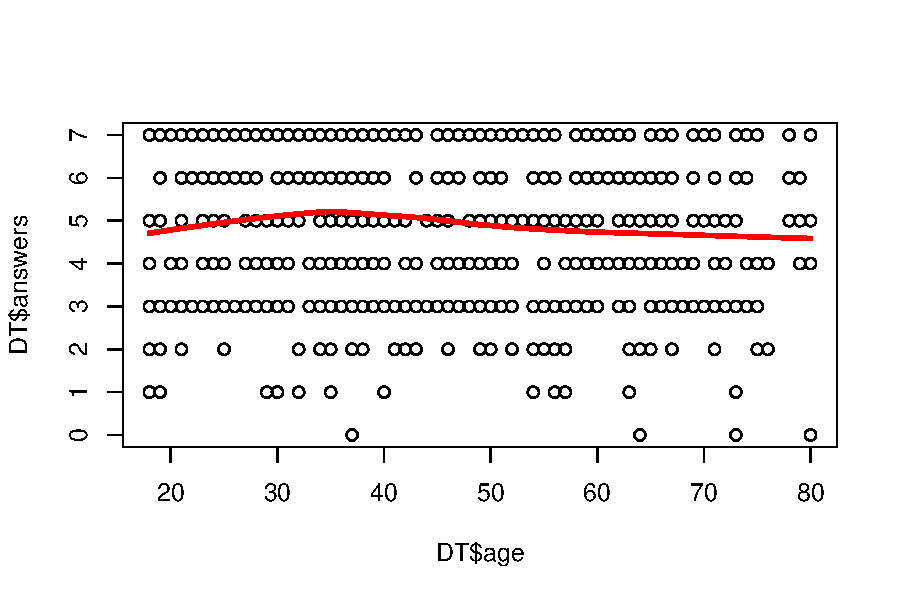
\includegraphics[width=\maxwidth]{figure/figure-6-2} 

}

\caption[Answers vs]{Answers vs. Age}\label{f:figure-62}
\end{figure}


\end{knitrout}


\newpage
\bibliography{004-bibliography}


\newpage
\appendix

\section{R Code}
\begin{knitrout}
\definecolor{shadecolor}{rgb}{0.969, 0.969, 0.969}\color{fgcolor}\begin{kframe}
\begin{alltt}
\hlkwd{plot}\hlstd{(DT}\hlopt{$}\hlstd{age, DT}\hlopt{$}\hlstd{answers)}
\hlkwd{lines}\hlstd{(stats}\hlopt{::}\hlkwd{lowess}\hlstd{(DT}\hlopt{$}\hlstd{age, DT}\hlopt{$}\hlstd{answers),} \hlkwc{col} \hlstd{=} \hlstr{"red"}\hlstd{,} \hlkwc{lwd} \hlstd{=} \hlnum{3}\hlstd{)}
\hlkwd{print}\hlstd{(}\hlkwd{sessionInfo}\hlstd{(),} \hlkwc{locale} \hlstd{=} \hlnum{FALSE}\hlstd{)}
\hlkwa{if} \hlstd{(}\hlopt{!}\hlkwd{require}\hlstd{(}\hlstr{"pacman"}\hlstd{))} \hlkwd{install.packages}\hlstd{(}\hlstr{"pacman"}\hlstd{)}

\hlstd{pacman}\hlopt{::}\hlkwd{p_load}\hlstd{(knitr, here, xtable, lattice, ggplot2, dplyr,}
    \hlstd{data.table, bookdown)}
\hlstd{multiplot} \hlkwb{<-} \hlkwa{function}\hlstd{(}\hlkwc{...}\hlstd{,} \hlkwc{plotlist} \hlstd{=} \hlkwa{NULL}\hlstd{,} \hlkwc{file}\hlstd{,} \hlkwc{cols} \hlstd{=} \hlnum{1}\hlstd{,} \hlkwc{layout} \hlstd{=} \hlkwa{NULL}\hlstd{) \{}
    \hlkwd{require}\hlstd{(grid)}

    \hlcom{# Make a list from the ... arguments and plotlist}
    \hlstd{plots} \hlkwb{<-} \hlkwd{c}\hlstd{(}\hlkwd{list}\hlstd{(...), plotlist)}

    \hlstd{numPlots} \hlkwb{=} \hlkwd{length}\hlstd{(plots)}

    \hlcom{# If layout is NULL, then use 'cols' to determine layout}
    \hlkwa{if} \hlstd{(}\hlkwd{is.null}\hlstd{(layout)) \{}
        \hlcom{# Make the panel ncol: Number of columns of plots nrow:}
        \hlcom{# Number of rows needed, calculated from # of cols}
        \hlstd{layout} \hlkwb{<-} \hlkwd{matrix}\hlstd{(}\hlkwd{seq}\hlstd{(}\hlnum{1}\hlstd{, cols} \hlopt{*} \hlkwd{ceiling}\hlstd{(numPlots}\hlopt{/}\hlstd{cols)),}
            \hlkwc{ncol} \hlstd{= cols,} \hlkwc{nrow} \hlstd{=} \hlkwd{ceiling}\hlstd{(numPlots}\hlopt{/}\hlstd{cols))}
    \hlstd{\}}

    \hlkwa{if} \hlstd{(numPlots} \hlopt{==} \hlnum{1}\hlstd{) \{}
        \hlkwd{print}\hlstd{(plots[[}\hlnum{1}\hlstd{]])}

    \hlstd{\}} \hlkwa{else} \hlstd{\{}
        \hlcom{# Set up the page}
        \hlkwd{grid.newpage}\hlstd{()}
        \hlkwd{pushViewport}\hlstd{(}\hlkwd{viewport}\hlstd{(}\hlkwc{layout} \hlstd{=} \hlkwd{grid.layout}\hlstd{(}\hlkwd{nrow}\hlstd{(layout),}
            \hlkwd{ncol}\hlstd{(layout))))}

        \hlcom{# Make each plot, in the correct location}
        \hlkwa{for} \hlstd{(i} \hlkwa{in} \hlnum{1}\hlopt{:}\hlstd{numPlots) \{}
            \hlcom{# Get the i,j matrix positions of the regions that contain}
            \hlcom{# this subplot}
            \hlstd{matchidx} \hlkwb{<-} \hlkwd{as.data.frame}\hlstd{(}\hlkwd{which}\hlstd{(layout} \hlopt{==} \hlstd{i,} \hlkwc{arr.ind} \hlstd{=} \hlnum{TRUE}\hlstd{))}

            \hlkwd{print}\hlstd{(plots[[i]],} \hlkwc{vp} \hlstd{=} \hlkwd{viewport}\hlstd{(}\hlkwc{layout.pos.row} \hlstd{= matchidx}\hlopt{$}\hlstd{row,}
                \hlkwc{layout.pos.col} \hlstd{= matchidx}\hlopt{$}\hlstd{col))}
        \hlstd{\}}
    \hlstd{\}}
\hlstd{\}}
\hlstd{dat} \hlkwb{<-} \hlkwd{read.table}\hlstd{(here}\hlopt{::}\hlkwd{here}\hlstd{(}\hlstr{"data"}\hlstd{,} \hlstr{"SOCATT.DAT"}\hlstd{),} \hlkwc{colClasses} \hlstd{=} \hlkwd{c}\hlstd{(}\hlstr{"factor"}\hlstd{,}
    \hlstr{"factor"}\hlstd{,} \hlstr{"numeric"}\hlstd{,} \hlstr{"numeric"}\hlstd{,} \hlstr{"numeric"}\hlstd{,} \hlstr{"numeric"}\hlstd{,} \hlstr{"numeric"}\hlstd{,}
    \hlstr{"numeric"}\hlstd{,} \hlstr{"numeric"}\hlstd{))}
\hlcom{# dat <- read.table('SOCATT.DAT', colClasses=c('factor',}
\hlcom{# 'factor', 'numeric', 'numeric', 'numeric', 'numeric',}
\hlcom{# 'numeric', 'numeric', 'numeric'))}
\hlkwd{colnames}\hlstd{(dat)} \hlkwb{<-} \hlkwd{c}\hlstd{(}\hlstr{"Districts"}\hlstd{,} \hlstr{"Subject"}\hlstd{,} \hlstr{"Year"}\hlstd{,} \hlstr{"Score"}\hlstd{,} \hlstr{"Party"}\hlstd{,}
    \hlstr{"SocialClass"}\hlstd{,} \hlstr{"Gender"}\hlstd{,} \hlstr{"Age"}\hlstd{,} \hlstr{"Religion"}\hlstd{)}
\hlstd{dat}\hlopt{$}\hlstd{Age_Cur} \hlkwb{<-} \hlstd{dat}\hlopt{$}\hlstd{Age} \hlopt{+} \hlstd{dat}\hlopt{$}\hlstd{Year} \hlopt{-} \hlnum{1}
\hlstd{dat}\hlopt{$}\hlstd{Year} \hlkwb{<-} \hlkwd{as.factor}\hlstd{(dat}\hlopt{$}\hlstd{Year} \hlopt{+} \hlnum{1982}\hlstd{)}
\hlstd{dat}\hlopt{$}\hlstd{Gender} \hlkwb{<-} \hlkwd{factor}\hlstd{(dat}\hlopt{$}\hlstd{Gender,} \hlkwc{labels} \hlstd{=} \hlkwd{c}\hlstd{(}\hlstr{"Male"}\hlstd{,} \hlstr{"Female"}\hlstd{))}
\hlstd{dat}\hlopt{$}\hlstd{Party} \hlkwb{<-} \hlkwd{factor}\hlstd{(dat}\hlopt{$}\hlstd{Party,} \hlkwc{labels} \hlstd{=} \hlkwd{c}\hlstd{(}\hlstr{"Conserv"}\hlstd{,} \hlstr{"Labour"}\hlstd{,}
    \hlstr{"Liberal"}\hlstd{,} \hlstr{"Other"}\hlstd{,} \hlstr{"None"}\hlstd{))}  \hlcom{# Liberal* = Liberal/SDP/Alliance}
\hlstd{dat}\hlopt{$}\hlstd{Religion} \hlkwb{<-} \hlkwd{factor}\hlstd{(dat}\hlopt{$}\hlstd{Religion,} \hlkwc{labels} \hlstd{=} \hlkwd{c}\hlstd{(}\hlstr{"Catholic"}\hlstd{,} \hlstr{"Protestant"}\hlstd{,}
    \hlstr{"Other"}\hlstd{,} \hlstr{"None"}\hlstd{))}
\hlstd{dat}\hlopt{$}\hlstd{SocialClass} \hlkwb{<-} \hlkwd{factor}\hlstd{(dat}\hlopt{$}\hlstd{SocialClass,} \hlkwc{labels} \hlstd{=} \hlkwd{c}\hlstd{(}\hlstr{"Middle"}\hlstd{,}
    \hlstr{"Upper"}\hlstd{,} \hlstr{"Lower"}\hlstd{))}
\hlstd{DT} \hlkwb{<-} \hlkwd{as.data.table}\hlstd{(}\hlkwd{read.table}\hlstd{(here}\hlopt{::}\hlkwd{here}\hlstd{(}\hlstr{"data"}\hlstd{,} \hlstr{"SOCATT.DAT"}\hlstd{)))}
\hlcom{# DT <- as.data.table(read.table('SOCATT.DAT'))}
\hlkwd{setnames}\hlstd{(DT,} \hlkwd{c}\hlstd{(}\hlstr{"District"}\hlstd{,} \hlstr{"id"}\hlstd{,} \hlstr{"year"}\hlstd{,} \hlstr{"answers"}\hlstd{,} \hlstr{"party"}\hlstd{,}
    \hlstr{"ses"}\hlstd{,} \hlstr{"sex"}\hlstd{,} \hlstr{"age"}\hlstd{,} \hlstr{"religion"}\hlstd{))}
\hlstd{DT[,} \hlkwd{`:=`}\hlstd{(}\hlkwc{party} \hlstd{=} \hlkwd{factor}\hlstd{(}\hlkwd{ifelse}\hlstd{(party} \hlopt{==} \hlnum{1}\hlstd{,} \hlstr{"Conserv"}\hlstd{,} \hlkwd{ifelse}\hlstd{(party} \hlopt{==}
    \hlnum{2}\hlstd{,} \hlstr{"Labour"}\hlstd{,} \hlkwd{ifelse}\hlstd{(party} \hlopt{==} \hlnum{3}\hlstd{,} \hlstr{"Liberal"}\hlstd{,} \hlkwd{ifelse}\hlstd{(party} \hlopt{==}
    \hlnum{4}\hlstd{,} \hlstr{"Other"}\hlstd{,} \hlstr{"None"}\hlstd{))))),} \hlkwc{answers.f} \hlstd{=} \hlkwd{factor}\hlstd{(answers,} \hlkwc{ordered} \hlstd{=} \hlnum{TRUE}\hlstd{),}
    \hlkwc{ses} \hlstd{=} \hlkwd{ifelse}\hlstd{(ses} \hlopt{==} \hlnum{1}\hlstd{,} \hlnum{2}\hlstd{,} \hlkwd{ifelse}\hlstd{(ses} \hlopt{==} \hlnum{2}\hlstd{,} \hlnum{3}\hlstd{,} \hlnum{1}\hlstd{)),} \hlkwc{sex} \hlstd{=} \hlkwd{factor}\hlstd{(}\hlkwd{ifelse}\hlstd{(sex} \hlopt{==}
        \hlnum{1}\hlstd{,} \hlstr{"Male"}\hlstd{,} \hlstr{"Female"}\hlstd{)),} \hlkwc{religion} \hlstd{=} \hlkwd{factor}\hlstd{(}\hlkwd{ifelse}\hlstd{(religion} \hlopt{==}
        \hlnum{1}\hlstd{,} \hlstr{"Catholic"}\hlstd{,} \hlkwd{ifelse}\hlstd{(religion} \hlopt{==} \hlnum{2}\hlstd{,} \hlstr{"Protestant"}\hlstd{,} \hlkwd{ifelse}\hlstd{(religion} \hlopt{==}
        \hlnum{3}\hlstd{,} \hlstr{"Other"}\hlstd{,} \hlstr{"None"}\hlstd{)))),} \hlkwc{year} \hlstd{=} \hlkwd{ifelse}\hlstd{(year} \hlopt{==} \hlnum{1}\hlstd{,} \hlnum{1983}\hlstd{,}
        \hlkwd{ifelse}\hlstd{(year} \hlopt{==} \hlnum{2}\hlstd{,} \hlnum{1984}\hlstd{,} \hlkwd{ifelse}\hlstd{(year} \hlopt{==} \hlnum{4}\hlstd{,} \hlnum{1985}\hlstd{,} \hlnum{1986}\hlstd{))))]}
\hlstd{DT[,} \hlkwd{`:=`}\hlstd{(}\hlkwc{ses} \hlstd{=} \hlkwd{factor}\hlstd{(}\hlkwd{ifelse}\hlstd{(ses} \hlopt{==} \hlnum{1}\hlstd{,} \hlstr{"lower"}\hlstd{,} \hlkwd{ifelse}\hlstd{(ses} \hlopt{==}
    \hlnum{2}\hlstd{,} \hlstr{"middle"}\hlstd{,} \hlstr{"upper"}\hlstd{)),} \hlkwc{ordered} \hlstd{= T))]}
\hlstd{g1} \hlkwb{<-} \hlkwd{ggplot}\hlstd{(}\hlkwc{data} \hlstd{= dat,} \hlkwd{aes}\hlstd{(}\hlkwc{x} \hlstd{= Year,} \hlkwc{y} \hlstd{= Score))} \hlopt{+} \hlkwd{geom_boxplot}\hlstd{()} \hlopt{+}
    \hlkwd{ggtitle}\hlstd{(}\hlstr{"Scores with different years"}\hlstd{)}  \hlcom{# http://en.wikipedia.org/wiki/The_Silent_Scream}
\hlstd{g2} \hlkwb{<-} \hlkwd{ggplot}\hlstd{(}\hlkwc{data} \hlstd{= dat,} \hlkwd{aes}\hlstd{(}\hlkwc{x} \hlstd{= Gender,} \hlkwc{y} \hlstd{= Score))} \hlopt{+} \hlkwd{geom_boxplot}\hlstd{()} \hlopt{+}
    \hlkwd{ggtitle}\hlstd{(}\hlstr{"Scores with different gender"}\hlstd{)}  \hlcom{# + facet_grid(. ~ Year) }
\hlstd{g3} \hlkwb{<-} \hlkwd{ggplot}\hlstd{(}\hlkwc{data} \hlstd{= dat,} \hlkwd{aes}\hlstd{(}\hlkwc{x} \hlstd{= Age,} \hlkwc{y} \hlstd{= Score))} \hlopt{+} \hlkwd{geom_point}\hlstd{()} \hlopt{+}
    \hlkwd{geom_smooth}\hlstd{(}\hlkwd{aes}\hlstd{(}\hlkwc{group} \hlstd{=} \hlnum{1}\hlstd{),} \hlkwc{method} \hlstd{=} \hlstr{"loess"}\hlstd{,} \hlkwc{size} \hlstd{=} \hlnum{2}\hlstd{)} \hlopt{+}
    \hlkwd{ggtitle}\hlstd{(}\hlstr{"Scores with different baseline ages"}\hlstd{)} \hlopt{+} \hlkwd{xlab}\hlstd{(}\hlstr{"Current Age"}\hlstd{)}  \hlcom{#  + facet_grid(. ~ Gender)}
\hlstd{g4} \hlkwb{<-} \hlkwd{ggplot}\hlstd{(}\hlkwc{data} \hlstd{= dat,} \hlkwd{aes}\hlstd{(}\hlkwc{x} \hlstd{= Party,} \hlkwc{y} \hlstd{= Score))} \hlopt{+} \hlkwd{geom_boxplot}\hlstd{()} \hlopt{+}
    \hlkwd{ggtitle}\hlstd{(}\hlstr{"Scores with different parties"}\hlstd{)}  \hlcom{# + facet_grid(. ~ Year)  + theme(axis.text.x = element_text(angle = 90, hjust = 1)) }
\hlstd{g5} \hlkwb{<-} \hlkwd{ggplot}\hlstd{(}\hlkwc{data} \hlstd{= dat,} \hlkwd{aes}\hlstd{(}\hlkwc{x} \hlstd{= SocialClass,} \hlkwc{y} \hlstd{= Score))} \hlopt{+} \hlkwd{geom_boxplot}\hlstd{()} \hlopt{+}
    \hlkwd{ggtitle}\hlstd{(}\hlstr{"Scores with different slcoal classes"}\hlstd{)}  \hlcom{# + facet_grid(. ~ Year) + theme(axis.text.x = element_text(angle = 90, hjust = 1)) }
\hlstd{g6} \hlkwb{<-} \hlkwd{ggplot}\hlstd{(}\hlkwc{data} \hlstd{= dat,} \hlkwd{aes}\hlstd{(}\hlkwc{x} \hlstd{= Religion,} \hlkwc{y} \hlstd{= Score))} \hlopt{+} \hlkwd{geom_boxplot}\hlstd{()} \hlopt{+}
    \hlkwd{ggtitle}\hlstd{(}\hlstr{"Scores with different religions"}\hlstd{)}  \hlcom{# + facet_grid(. ~ Year) + theme(axis.text.x = element_text(angle = 90, hjust = 1)) }
\hlkwd{multiplot}\hlstd{(g1, g2, g3, g4, g5, g6,} \hlkwc{cols} \hlstd{=} \hlnum{2}\hlstd{)}
\hlkwd{set.seed}\hlstd{(}\hlnum{123455}\hlstd{)}
\hlstd{sample.id} \hlkwb{<-} \hlkwd{sample}\hlstd{(}\hlkwd{unique}\hlstd{(DT}\hlopt{$}\hlstd{id),} \hlnum{30}\hlstd{)}
\hlkwd{xyplot}\hlstd{(answers} \hlopt{~} \hlkwd{factor}\hlstd{(year),} \hlkwc{group} \hlstd{= id,} \hlkwc{data} \hlstd{= DT[id} \hlopt
    \hlstd{sample.id],} \hlkwc{type} \hlstd{=} \hlkwd{c}\hlstd{(}\hlstr{"l"}\hlstd{,} \hlstr{"p"}\hlstd{),} \hlkwc{lty} \hlstd{=} \hlnum{2}\hlstd{,} \hlkwc{xlab} \hlstd{=} \hlstr{"year"}\hlstd{,} \hlkwc{ylab} \hlstd{=} \hlstr{"score"}\hlstd{,}
    \hlkwc{aspect} \hlstd{=} \hlstr{"xy"}\hlstd{,} \hlkwc{main} \hlstd{=} \hlstr{"response profiles for a random sample of 30 subjects"}\hlstd{)}
\hlkwd{xyplot}\hlstd{(answers} \hlopt{~} \hlkwd{factor}\hlstd{(year),} \hlkwc{group} \hlstd{= id,} \hlkwc{data} \hlstd{= DT[id} \hlopt
    \hlstd{sample.id],} \hlkwc{type} \hlstd{=} \hlkwd{c}\hlstd{(}\hlstr{"r"}\hlstd{),} \hlkwc{aspect} \hlstd{=} \hlstr{"xy"}\hlstd{,} \hlkwc{xlab} \hlstd{=} \hlstr{"year"}\hlstd{,}
    \hlkwc{ylab} \hlstd{=} \hlstr{"score"}\hlstd{,} \hlkwc{index.cond} \hlstd{=} \hlkwa{function}\hlstd{(}\hlkwc{x}\hlstd{,} \hlkwc{y}\hlstd{)} \hlkwd{coef}\hlstd{(}\hlkwd{lm}\hlstd{(y} \hlopt{~} \hlstd{x))[}\hlnum{1}\hlstd{],}
    \hlkwc{main} \hlstd{=} \hlstr{"Least squares fits (with year) for the same random sample of 30 subjects"}\hlstd{)}
\hlstd{m} \hlkwb{<-} \hlkwd{ggplot}\hlstd{(DT,} \hlkwd{aes}\hlstd{(}\hlkwc{x} \hlstd{= answers))}

\hlstd{m} \hlopt{+} \hlkwd{geom_histogram}\hlstd{(}\hlkwd{aes}\hlstd{(}\hlkwc{y} \hlstd{= ..density..),} \hlkwc{binwidth} \hlstd{=} \hlnum{1}\hlstd{,} \hlkwc{colour} \hlstd{=} \hlstr{"darkgreen"}\hlstd{,}
    \hlkwc{fill} \hlstd{=} \hlstr{"white"}\hlstd{)} \hlopt{+} \hlkwd{facet_grid}\hlstd{(party} \hlopt{~} \hlstd{year)} \hlopt{+} \hlkwd{labs}\hlstd{(}\hlkwc{title} \hlstd{=} \hlstr{"Response by year and political party"}\hlstd{)}

\hlstd{m} \hlopt{+} \hlkwd{geom_histogram}\hlstd{(}\hlkwd{aes}\hlstd{(}\hlkwc{y} \hlstd{= ..density..),} \hlkwc{binwidth} \hlstd{=} \hlnum{1}\hlstd{,} \hlkwc{colour} \hlstd{=} \hlstr{"darkgreen"}\hlstd{,}
    \hlkwc{fill} \hlstd{=} \hlstr{"white"}\hlstd{)} \hlopt{+} \hlkwd{facet_grid}\hlstd{(ses} \hlopt{~} \hlstd{year)} \hlopt{+} \hlkwd{labs}\hlstd{(}\hlkwc{title} \hlstd{=} \hlstr{"Response by year and SES"}\hlstd{)}

\hlstd{m} \hlopt{+} \hlkwd{geom_histogram}\hlstd{(}\hlkwd{aes}\hlstd{(}\hlkwc{y} \hlstd{= ..density..),} \hlkwc{binwidth} \hlstd{=} \hlnum{1}\hlstd{,} \hlkwc{colour} \hlstd{=} \hlstr{"darkgreen"}\hlstd{,}
    \hlkwc{fill} \hlstd{=} \hlstr{"white"}\hlstd{)} \hlopt{+} \hlkwd{facet_grid}\hlstd{(religion} \hlopt{~} \hlstd{year)} \hlopt{+} \hlkwd{labs}\hlstd{(}\hlkwc{title} \hlstd{=} \hlstr{"Response by year and religion"}\hlstd{)}
\end{alltt}
\end{kframe}
\end{knitrout}

\newpage

\section{Session Information}
\begin{knitrout}
\definecolor{shadecolor}{rgb}{0.969, 0.969, 0.969}\color{fgcolor}\begin{kframe}
\begin{alltt}
\hlkwd{print}\hlstd{(}\hlkwd{sessionInfo}\hlstd{(),} \hlkwc{locale} \hlstd{=} \hlnum{FALSE}\hlstd{)}
\end{alltt}
\begin{verbatim}
## R version 3.6.0 (2019-04-26)
## Platform: x86_64-pc-linux-gnu (64-bit)
## Running under: Pop!_OS 18.10
## 
## Matrix products: default
## BLAS:   /usr/lib/x86_64-linux-gnu/blas/libblas.so.3.8.0
## LAPACK: /usr/lib/x86_64-linux-gnu/lapack/liblapack.so.3.8.0
## 
## attached base packages:
## [1] grid      stats     graphics  grDevices utils    
## [6] datasets  methods   base     
## 
## other attached packages:
## [1] bookdown_0.9      data.table_1.12.0 dplyr_0.8.0.1    
## [4] ggplot2_3.1.0     lattice_0.20-38   xtable_1.8-4     
## [7] here_0.1          pacman_0.5.0      knitr_1.22       
## 
## loaded via a namespace (and not attached):
##  [1] Rcpp_1.0.1       magrittr_1.5     tidyselect_0.2.5
##  [4] munsell_0.5.0    colorspace_1.4-0 R6_2.4.0        
##  [7] rlang_0.3.4      highr_0.8        stringr_1.4.0   
## [10] plyr_1.8.4       tools_3.6.0      gtable_0.2.0    
## [13] xfun_0.6         withr_2.1.2      lazyeval_0.2.1  
## [16] rprojroot_1.3-2  assertthat_0.2.1 tibble_2.1.1    
## [19] crayon_1.3.4     reshape2_1.4.3   formatR_1.6     
## [22] purrr_0.3.2      glue_1.3.1       evaluate_0.13   
## [25] labeling_0.3     stringi_1.4.3    compiler_3.6.0  
## [28] pillar_1.3.1     scales_1.0.0     backports_1.1.3 
## [31] pkgconfig_2.0.2
\end{verbatim}
\end{kframe}
\end{knitrout}


\end{document}
